
\documentclass[xcolor=table]{beamer}

% for fancy Mike style table
 \usepackage[table]{xcolor} 
 \usepackage{multirow}
\usepackage{textpos}
\usepackage{helvet}
\usepackage{caption}
\usepackage{changepage}
\usepackage{algorithmic}
\usepackage{array}
\setbeamerfont{caption}{size = \footnotesize}
\usepackage{multicol}
\usepackage{setspace}

% useful packages for including code
\usepackage{listings}
\usepackage{color}
\lstset{breaklines}

% package for drawing graphs
\usepackage{tikz}
\usetikzlibrary{positioning}

\definecolor{charlesBlue}{RGB}{100, 155, 255}
\definecolor{charlesBlue2}{RGB}{0, 155, 255}
\definecolor{MRGGreen}{rgb}{0, 0.350, 0.200}
\usecolortheme{default}

% References
%\bibliographystyle{apacite} 
\hypersetup{colorlinks = true, linkcolor={MRGGreen}, citecolor = black, urlcolor = blue}


% Custom colors for alerts and examples
\setbeamercolor{palette primary}{fg=MRGGreen}
\setbeamercolor{palette secondary}{fg=MRGGreen}
\setbeamercolor{palette tertiary}{bg= MRGGreen}
\setbeamercolor*{structure}{fg=MRGGreen}
\setbeamercolor{titlelike}{fg=black}

\lstset{
  basicstyle=\tiny \ttfamily,
  columns=fullflexible,
}

\setbeamertemplate{bibliography item}[text]
\title[Stan workshop 2019]{\textcolor{MRGGreen}{Population and ODE-based models \\
 using Stan and Torsten}}

%\author{Charles Margossian} 
%\institute{Columbia University, Department of Statistics} 
\date{Stan Con 2019, \\ Cambridge, UK}

\captionsetup{font=scriptsize,labelfont=scriptsize, labelformat=empty}


\begin{document} 

\begin{frame}
  \begin{textblock*}{80mm}(-2mm,0mm)
  \end{textblock*}
  \begin{textblock*}{80mm}(0.7\textwidth,0.7\textheight)
    
\includegraphics[width=0.25\textwidth]{../torstenLogo.png}
    
\includegraphics[width=0.25\textwidth]{../stanLogo.png}
  \end{textblock*}
  \titlepage
\end{frame}

\begin{frame}
  Instructors:
  \begin{itemize}
    \item {Charles Margossian \\ Columbia University, Department of Statistics}
    \item {Yi Zhang \\ Metrum Research Group}
  \end{itemize}
  
\end{frame}

\begin{frame}
  \frametitle{Outline}

   Day 1
   \begin{itemize}
     \item Introduction and modeling framework
     \item Pharmacometrics models
     \item Ordinary differential equation(ODE) based models
     \item Numerical ODE integrators
   \end{itemize}
   
   \ \\
   Day 2
   \begin{itemize}
     \item Population models
     \item Group/Population ODE integrators and MPI parallelisation
     \item Group/Population solvers
   \end{itemize}
\end{frame}


\begin{frame}
  \frametitle{Logistics}
  
  We use the the cloud platform \textit{Metworx}
  which has all the requisite files and softwares installed. \\ \ \\ \ \\
  
  \begin{center}
    
\includegraphics[width=3cm]{../metworx}
  \end{center}

  \begin{figure}
    \centering
    \begin{minipage}{0.3\textwidth}
      \centering
      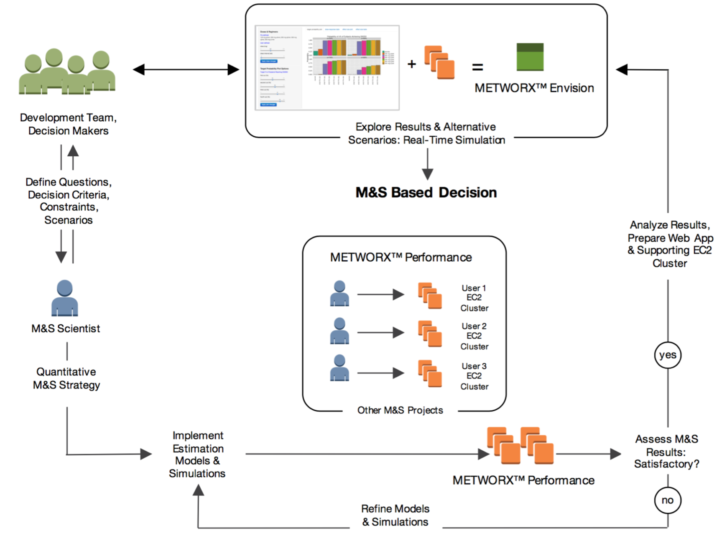
\includegraphics[width=0.9\textwidth]{./metworx_efficiencies}
    \end{minipage}
    \begin{minipage}{0.3\textwidth}
      \centering
      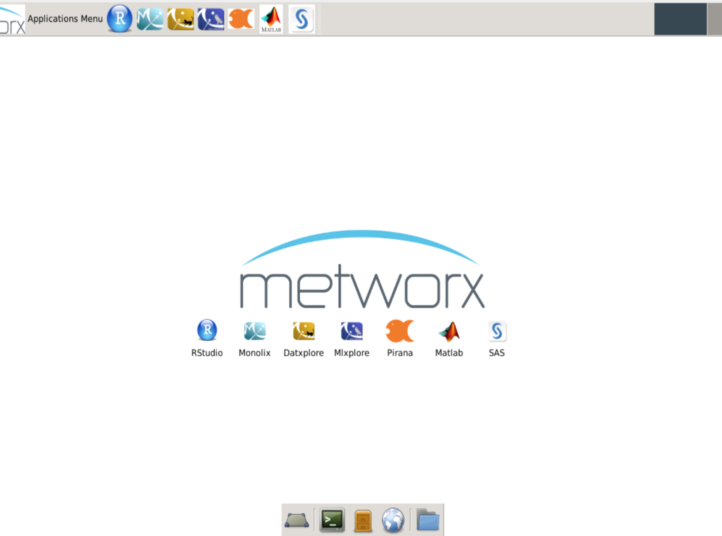
\includegraphics[width=0.9\textwidth]{./metworx_desktop}
    \end{minipage}
    \begin{minipage}{0.3\textwidth}
      \centering
      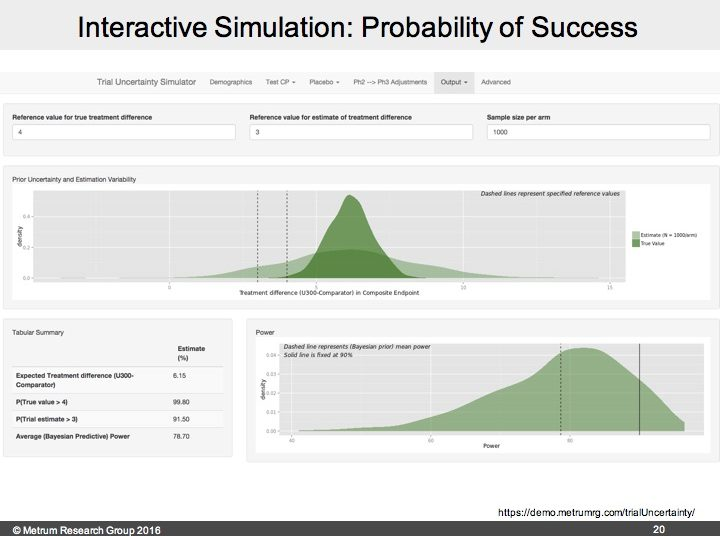
\includegraphics[width=0.9\textwidth]{./metworx_decisionmakingtools}
    \end{minipage}
  \end{figure}
  
\end{frame}

\begin{frame}
  \frametitle{Logistics}

  The workshop package includes:
  \begin{itemize}
    \item R scripts and Stan files to do the exercises
    \item These slides
    \item Outline of the course
    \item Additional documentation
  \end{itemize}
  
  \ \\
  We will be using:
  \begin{itemize}
    \item Torsten v0.87
    \item RStan v2.19.2
    \item ggplot, plyr, tidyr, dplyr
  \end{itemize}

\end{frame}

\begin{frame}
  \begin{center}
    {\Large I} \\ \ \\ Introduction and modeling framework
  \end{center}
\end{frame}

\begin{frame}
  \frametitle{Preliminary question}
  \begin{itemize}
    \item Why Bayesian in a field such as pharmacometrics?
    \item Example - \textit{Bayesian aggregation of average data: an application
      in drug development} \cite{Weber:2018}.
  \end{itemize}
\end{frame}

\begin{frame}
  \frametitle{Modeling framework}
  
  Box's loop:
  
  \begin{figure}[htbp]
  \begin{center}
  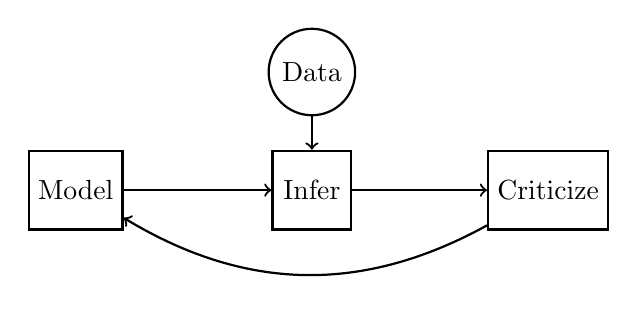
\begin{tikzpicture}
  [
    Box/.style={rectangle, draw=black!, fill=green!0, thick, minimum size=10mm},
    Gray/.style={rectangle, draw=black!, fill=gray!35, thick, minimum size=1mm},
    Round/.style={circle, draw=black!, fill=green!0, thick, minimum size=1mm},
  ]
  % Nodes
  \node[Round] (Data) at(0, 1.5) {Data};
  \node[Box] (Model) at(-3, 0) {Model};
  \node[Box] (Infer) at(0, 0) {Infer};
  \node[Box] (Crit) at (3, 0) {Criticize};

  % Lines
  \path [->, draw, thick] (Model) -- (Infer);
  \path [->, draw, thick] (Infer) -- (Crit);
  \path [->, draw, thick] (Crit) edge[bend left] (Model);
  \path [->, draw, thick] (Data) -- (Infer);
 
 % 
  
  \end{tikzpicture}
  \end{center}
  \end{figure}

\end{frame}

\begin{frame}
  \frametitle{Inference}

  \begin{itemize}
    \item find the set of parameters consistent with our model and our data
    \item approximate this set with draws from the posterior distribution
  \end{itemize}

\end{frame}

\begin{frame}
  \frametitle{Sampling algorithm}
  
  \begin{itemize}
    \item Use the NUTS to sample $\pi (\theta | y)$
    \item Requires users the specify $\log \pi(\theta, y) = \log \pi(y | \theta) + \log \pi(\theta)$
  \end{itemize}

\end{frame}

\begin{frame}
  \frametitle{The ``criticism'' step}
  
  This step can be broken up in two parts:
  \begin{enumerate}
    \item did we sample from the correct distribution?
    \item does our model capture the characteristics of the data we care about?
  \end{enumerate}

\end{frame}

\begin{frame}
  \frametitle{Diagnosing the inference algorithm}
  \begin{itemize}
    \item look at the trace and the density plots
    \item look at $\hat R$ and effective number of samples
    \item have any warning messages been issued, i.e. divergent transitions ?
  \end{itemize}

\end{frame}

\begin{frame}
  \frametitle{Example: fitting a linear model}

  Likelihood:
  \begin{eqnarray*}
    Y & \sim & \mathrm{Normal}(x \beta, \sigma^2)
  \end{eqnarray*}

  Prior:
  \begin{eqnarray*}
    \beta & \sim & \mathrm{Normal}(2, 1) \\
    \sigma^2 & \sim & \mathrm{Normal}(1, 1)
  \end{eqnarray*}

\end{frame}

\begin{frame}
  \begin{itemize}
    \item No warning messages.
  \end{itemize}
  \begin{center}
    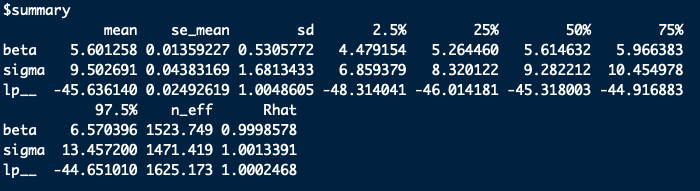
\includegraphics[width=4.5in]{../figures/linear_summary}
  \end{center}
\end{frame}

\begin{frame}
  \frametitle{Trace plots}
  \begin{center}
    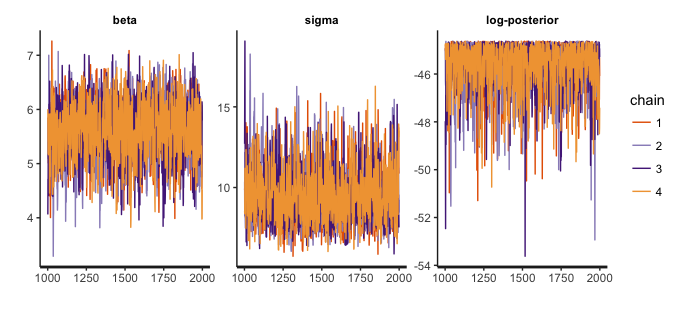
\includegraphics[width=3in]{../figures/linear_trace.png}
  \end{center}
\end{frame}

\begin{frame}
  \frametitle{Density plots}
  \begin{center}
    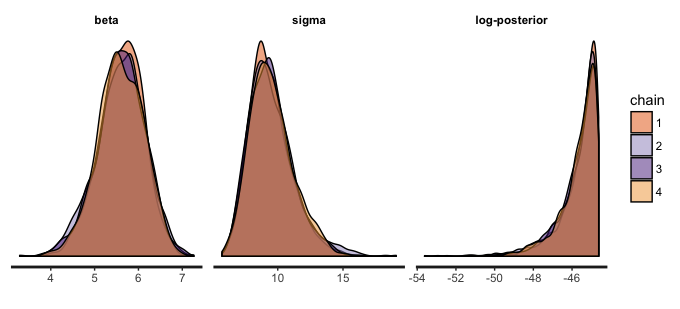
\includegraphics[width=3in]{../figures/linear_dens_plot.png}
  \end{center}
\end{frame}

\begin{frame}
  \frametitle{Posterior predictive checks}
  \begin{center}
    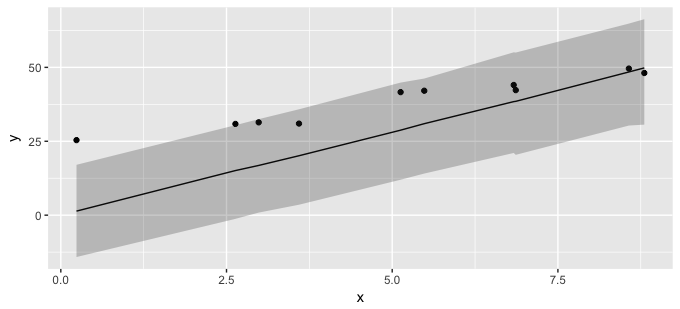
\includegraphics[width=3in]{../figures/linear_pred.png}
  \end{center}
\end{frame}

\begin{frame}
  \frametitle{So, how can we improve the model?}

  Likelihood:
  \begin{eqnarray*}
    Y & \sim & \mathrm{Normal}(x \beta, \sigma^2)
  \end{eqnarray*}

  Prior:
  \begin{eqnarray*}
    \beta & \sim & \mathrm{Normal}(2, 1) \\
    \sigma^2 & \sim & \mathrm{Normal}(1, 1)
  \end{eqnarray*}

\end{frame}

\begin{frame}
  \frametitle{Further reading}

  \begin{itemize}
    \item Philosophy and the practice of Bayesian statistics \cite{Gelman:2013b}
    \item Build, Compute, Critique, Repeat: Data Analysis with Latent Variable Models \cite{Blei:2014}
    \item Visualization in Bayesian workflow \cite{Gabry:2017}
    \item Towards a principled Bayesian workflow \cite{Betancourt:2018}
  \end{itemize}

\end{frame}


\section{References}
\begin{frame}[allowframebreaks]{References}
\scriptsize
% \bibliographystyle{unsrt}
%\bibliographystyle{authoryear}
\bibliographystyle{apalike}
\bibliography{../ref}  
\end{frame}

\end{document}
